\documentclass[12pt]{article}

\usepackage{sbc-template}
\usepackage{graphicx,url}

\usepackage[brazil]{babel}   
\usepackage[utf8]{inputenc}  
\usepackage{float}
\usepackage{subfigure}
     
\sloppy

\title{Relatório Trabalho 2 - PIHS}

\author{Guilherme Zamberlam Pomini  RA: 99345\inst{1} Diogo Fernando de Melo Sales RA: 93814 \inst{1}}

\address{Professor: Ronaldo Augusto de Lara Gonçalves \\ Disciplina: Programação para Interfaceamento de Hardware e Software \\ Ciência da Computação \\Universidade Estadual de Maringá (UEM) \\ Sede Maringá -- Paraná -- Brasil\email{ra99345@uem.br, ra93814@uem.br}}

\begin{document} 

\maketitle

\begin{figure}[H]
\centering

\includegraphics[width=.5\textwidth]{Imagens/logo.png}
\end{figure}


\section*{Introdução e Objetivo}

O presente documento contém relatório do segundo trabalho da matéria ministrada pelo Ronaldo Augusto de Lara Gonçalves na disciplina de Programação para Interfaceamento de Hardware e Software para a turma de Bacharelado em Ciência da Computação no primeiro semestre de 2018.

O objetido do segundo trabalho era implementar um programa em linguagem Assembly padrão 32 bits que lesse uma expressão matemática digitada pelo usuário, a interpretasse e a resolvesse, similar ao funcionamento de uma calculadora científica padrão. Similarmente a uma calculadora o programa deve fazer o tratamento de prioridade de operações, funções e sub-expressões delimitadas por parênteses.

A expressão matemática pode conter tanto operações básicas como soma, subtração, multiplicação e divisão, quanto operações matemáticas mais complexas como potências, raíz quadrada, logaritmos na base 10 e funções trigonométricas como seno, cosseno e tangente. Pode-se colocar parênteses como forma de controlar as prioridades das operações mas as funções não aceitam argumentos complexos. A expressão trabalha com números reais, dando o resultado portanto em um número real com ponto flutuante, mas também aceita números inteiros normalmente.

\section*{Principais Componentes}

O programa desenvolvido possui dois arquivos de códigos principais, um arquivo em linguagem C e Assembly 32 bits chamado principal, e um arquivo em linguagem Assembly 32 bits chamado calcexpress.

A funcionalidade do arquivo principal.c é realizar a leitura de uma expressão utilizando Assembly Inline e chamadas ao sistema, sem chamadas a bibliotecas e resolver a expressão utilizando Assembly Outline. A leitura da expressão é feita com a função le\_expressao como mostra a Figura~\ref{le_expressao}

\begin{figure}[H]
\centering
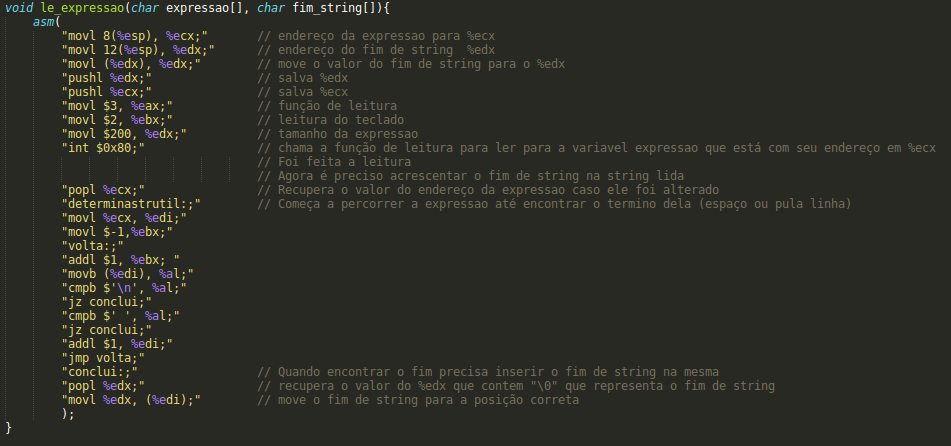
\includegraphics[width=\textwidth]{Imagens/le_expressao.png}
\caption{Função le\_expressao}
\label{le_expressao}
\end{figure}

A função é implementada com Assembly Inline e somente chamadas ao sistema, consiste primeiramente em ler uma expressão digitada pelo usuário para o endereço da string passada como parâmetro. Feita a leitura é necessário encontrar o fim da expressão e colocar um caractere simbolizando o fim de de string, finalizando a função.

O corpo main do arquivo principal.c como mostra a Figura~\ref{principal} consiste da declaração das variáveis para armazenar a expressão e a resposta, de prints para o usuário do funcionamento do programa, chamada da função para ler a expressão e chamada outline para resolver a expressão implementada no arquivo calcexpress.s

\begin{figure}[H]
\centering
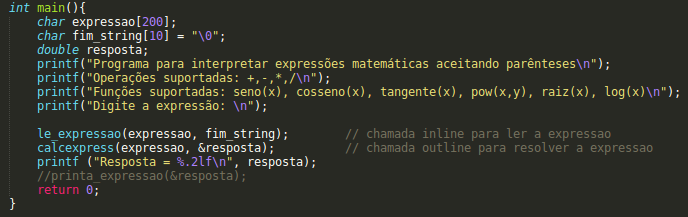
\includegraphics[width=\textwidth]{Imagens/principal.png}
\caption{Main arquivo principal.c}
\label{principal}
\end{figure}

Funcionalidades do arquivo calcexpress.s :

\begin{itemize}

\item \textbf{calcexpress} é o procedimento que o programa principal chama para resolver a expressão, é passado como parâmetro uma string que é a expressão a ser resolvida e um endereço de um double onde vai ser escrito o resultado. É este o procedimento que chama os demais procedimentos de criar uma lista duplamente encadeada a partir da expressão e o de resolve-la. A Figura~\ref{calcexpress} mostra as funcionalidades do procedimento.

\begin{figure}[H]
\centering
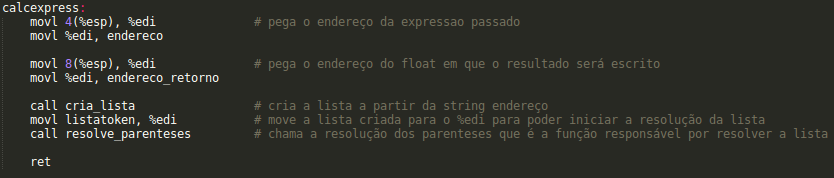
\includegraphics[width=\textwidth]{Imagens/calcexpress.png}
\caption{Procedimento calcexpress}
\label{calcexpress}
\end{figure}

\item \textbf{cria\_lista} procedimento para transformar a expressão em forma de string para uma lista duplamente encadeada, recebe o endereço da string lida pelo procedimento ler\_expressao no programa principal e passada para o procedimento calcexpress. Realiza a leitura caractere por caractere da expressão, faz os tratamentos necessários como resolver as funções, ler os números e operadores matemáticos. É o procedimento que converte os números em forma de String para ponto flutuante antes de fazer a inserção dos mesmos na lista. Ao final desse procedimento todas as funções foram resolvidas e seus resultados já estão em formato ponto flutuante como um elemento da lista, restando uma lista duplamente encadeada onde seus elementos são somente números reais, operadores matemáticos (+,-,/,*) e parênteses.

\item \textbf{resolve\_parenteses} procedimento que faz a varredura da lista procurando sub-expressões delimitadas por abre e fecha parênteses para serem resolvidas. A cada sub-expressão encontrada o procedimento chama o procedimento reduz para resolver somente o pedaço da lista correspondente a sub-expressão. Terminado a resolução de todos os parênteses é chamado novamente o procedimento reduz para resolver o restante da lista desde o começo.

\item \textbf{reduz} procedimento principal para resolução da expressão, recebe um endereço da lista que é passado pelo procedimento resolve\_parenteses e a resolve até chegar em um final de lista. A resolução é feita sequencialmente em três passadas pela lista, primeiramente tratando os números, em seguida as multiplicações e divisões e por fim as somas e subtrações. A cada tratamento de operações a lista vai sendo reduzida até sobrar somente um único elemento que é o resultado da expressão.

\end{itemize}

\section*{Funcionamento}

A primeira parte do programa se da no arquivo principal.c. É nele que é chamado a função le\_expressao que utiliza de Assembly Inline para ler a expressão digitada pelo usuário utilizando somente chamadas ao sistema. Após a leitura o programa chama a função calcexpress para resolver a expressão, por ser um procedimento onde sua definição está no arquivo calcexpress.s, esta é uma chamada utilizando Assembly Outline.

Dentro do procedimento calcexpress será resolvida a expressão com o primeiro passo sendo transformar a mesma para uma lista duplamente encadeada onde cada número e operação é um elemento da lista. Os elementos da lista são da forma de 20 bits, sendo 4 para o tipo do elemento, 8 para o valor, 4 para o endereço do elemento anterior e 4 para o endereço do elemento posterior. A conversão é feita por um método cria\_lista que vai percorrer a expressão caractere por caractere para reconhecer se é um número, operação ou uma função e realiza o seu respectivo tratamento.

A função cria\_lista possui um tratamento para cada tipo de elemento encontrado antes de fazer a inserção na lista de fato. Quando encontrado um caractere númerico o mesmo é lido até o fim e convertido para ponto flutuante independente se é um número inteiro ou número real. Quando encontrado uma operação matemática básica a mesma é inserida normalmente na lista sem necessidade de conversão. O tratamento das funções como Logaritmo, Raíz, Potência, Seno, Cosseno e Tangente é o mesmo, é encontrado o seu valor dentro dos respectivos parênteses, convertido para para ponto flutuante e calculado a sua função, sendo essa a única parte que realmente difere de fato pois cada função possui uma chamada diferente para o seu cálculo. Como o cálculo das funções é feito na hora de criar a lista, o que é inserido na lista é o seu valor de fato como um número real, portanto as funções são resolvidas no momento da criação da lista.

Após a criação da lista é necessário resolve-la, se fosse uma expressão normal bastaria chamar a função reduz. Contudo, como a expressão pode ou não conter sub-expressões que delimitam prioridades sobre outras operações o primeiro passo para resolver a lista é encontrar tais sub-expressões.

Tal problema é resolvido com o procedimento resolve\_parenteses que percorre a expressão resolvendo as suas sub-expressões até chegar no momento em que todos os parênteses foram eliminados, e resolvendo a expressão restante para dar o resultado desejado. O procedimento se baseia em percorrer a expressão até encontrar um token simbolizando um fecha parênteses, quando encontrado é chamado o método reduz que resolve expressões para resolver somente entre o endereço do último abre parênteses até o fecha parênteses encontrado, retirando todos os elementos utilizados e substituindo pelo resultado. A cada sub-expressão resolvida o procedimento começa a varredura do começo da lista, sempre garantindo pegar as sub-expressões mais aninhadas que possuem maior prioridade sobre as outras.

O procedimento reduz tem o objetivo de reduzir a lista a somente um elemento que seria o resultado da expressão. Recebe como endereço inicial o endereço de uma parte da expressão passada pelo método resolve\_parenteses, a resolvendo até encontrar o fim da lista passada. Consiste em três passadas pela lista, a primeira fazendo o tratamento dos números negativos, encontrando um token de menos e um número após e transformando em somente um elemento que seria o número negativado. A segunda passada resolve somente divisões e multiplicações por terem prioridade sobre a soma, resolvendo na ordem que as mesmas vão aparecendo. E por fim a terceira passada sobre a lista termina resolvendo as somas e subtrações que são as únicas operações restantes.

Tanto na segunda passada quanto na terceira o método de resolução é o mesmo, após encontrar uma operação entre dois números os mesmos são enviados para a pilha de ponto flutuante (FPU) e é identificada a operação, chamando seu respectivo tratamento através da FPU. Após computado o resultado o mesmo é sobrescrito no endereço do primeiro operando da operação e os dois elementos posteriores (a operação e o segundo operando) são retirados da lista através da manipulação dos seus ponteiros. Tal repetição de retirada da lista vai levar a um momento em que só existirá um único elemento na lista, o resultado esperado da expressão. 

Portanto, a resolução da lista é baseada nos métodos resolve\_parenteses que encontra as sub-expressões para serem resolvidas (a expressão sem parênteses é uma sub-expressão própria) utilizando o método reduz. Ao final o resultado será o único elemento da lista que será passado para o endereço de retorno do procedimento calcexpress para ser printado pelo usuário no programa principal.

\section*{Capacidades e Limitações}

Lista das capacidades do programa:

\begin{enumerate}
\item Leitura da expressão com Assembly Inline;
\item Resolução da expressão com Assembly Outline;
\item Tratamento para números em ponto flutuante, aceitando tanto inteiros quanto números reais e tratando os dois da mesma forma (como ponto flutuante) através da mesma conversão;
\item Tratamento prioridade de sub-expressões delimitadas por parênteses;
\item Trata espaços em branco como divisão entre elementos na escrita da expressão;
\item Trata precedência de operações, resolvendo primeiramente as funções enquanto cria a lista, multiplicação e divisão, e por fim soma e subtração.
\item Soma de dois números reais;
\item Subtração de dois números reais;
\item Divisão de dois números reais;
\item Multiplicação de dois números reais;
\item Potência na forma x elevado a y;
\item Raíz quadrada de um número real;
\item Logaritmo na base 10 de um número real;
\item Seno de um número real (passado em forma de radianos);
\item Cosseno de um número real (passado em forma de radianos);
\item Tangente de um número real (passado em forma de radianos);
\item Tratamento para números negativos.
\end{enumerate}

E as limitações do programa são:

\begin{enumerate}

\item Falta de uma função para verificar a ordem dos elementos da lista, para cancelar a execução caso os elementos não estejam da forma experada para a resolução;

\item A expressão deve possuir um tamanho máximo de 200 caracteres;

\item Não são aceitos argumentos compostos para expressões como da forma raiz(10+10);

\item O print do resultado final não é feito com chamada ao sistema por não ter sido encontrado uma maneira de printar um float sem chamadas de bibliotecas, fica como sugestão para melhoria do trabalho numa futura atualização.

\end{enumerate}

\section*{Conclusão}

O objetivo deste trabalho era implementar um interpretador de expressões matemáticas em linguagem Assembly 32 bits que trabalhasse tanto com  operações básicas quanto algumas mais complexas, realizando também o tratamento de prioridades de sub-expressões através de parênteses. O programa deveria ser dividido em duas partes, a primeira realizando a leitura da expressão com Assembly Inline e a segunda sendo um procedimento Assembly Outline para resolver a expressão.

Ao final do trabalho foi possível chegar no resultado esperado produzindo um programa nas especificações desejadas, salvo as limitações listadas, que resolve desde expressões simples até as mais complexas com prioridades. A Figura~\ref{resultado} mostra a resolução da expressão ${(2^{2} -2)*10-(\sqrt{16}/({\log_{10} 100}+1) }$ como era de se esperar de uma calculadora.

\begin{figure}[H]
\centering
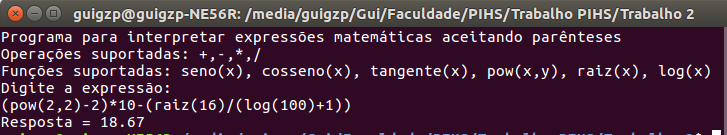
\includegraphics[width=\textwidth]{Imagens/resolvido.png}
\caption{Resolução expressão}
\label{resultado}
\end{figure}


\nocite{*}

\bibliographystyle{sbc}
\bibliography{Referencias}

\end{document}

